% =====================================================================
% Documentación Técnica — Evaluación Técnica Jaguar de México
% Candidato: Ing. Jair Molina Arce
% Sistema de Extracción de Aire Caliente para Gabinete de Telecom
% Compilar: pdflatex (x2) — MiKTeX
% =====================================================================
\documentclass[11pt,letterpaper]{article}

\usepackage[utf8]{inputenc}
\usepackage[T1]{fontenc}
\usepackage[spanish,es-noshorthands]{babel}
\usepackage{lmodern}
\usepackage{microtype}
\usepackage[margin=2.5cm,headheight=14pt]{geometry}
\usepackage{graphicx}
\usepackage[table]{xcolor}
\usepackage{booktabs}
\usepackage{tabularx}
\usepackage{longtable}
\usepackage{array}
\usepackage{enumitem}
\usepackage{titlesec}
\usepackage{fancyhdr}
\usepackage{caption}
\usepackage{float}
\usepackage{amsmath}
\usepackage[hidelinks,pdfusetitle]{hyperref}

% ------------------ Paleta corporativa ------------------
\definecolor{JagDark}{HTML}{0F3057}   % azul petróleo oscuro
\definecolor{JagMid}{HTML}{00587A}    % azul medio
\definecolor{JagAccent}{HTML}{008891} % teal
\definecolor{JagGray}{HTML}{5C6B73}   % gris técnico
\definecolor{RowGray}{HTML}{F0F4F5}

% ------------------ Estilo de secciones ------------------
\titleformat{\section}
  {\Large\bfseries\color{JagDark}}{\thesection.}{0.6em}{}
  [\vspace{-0.6em}{\color{JagAccent}\rule{\textwidth}{0.9pt}}]
\titleformat{\subsection}
  {\large\bfseries\color{JagMid}}{\thesubsection}{0.6em}{}
\titleformat{\subsubsection}
  {\normalsize\bfseries\color{JagGray}}{\thesubsubsection}{0.6em}{}

% ------------------ Encabezado / pie ------------------
\pagestyle{fancy}
\fancyhf{}
\fancyhead[L]{\small\color{JagGray}Evaluación Técnica --- Sistemas Embebidos Jr.}
\fancyhead[R]{\small\color{JagGray}Jaguar de México}
\fancyfoot[L]{\small\color{JagGray}Ing. Jair Molina Arce}
\fancyfoot[R]{\small\color{JagGray}Página \thepage}
\renewcommand{\headrulewidth}{0.4pt}
\renewcommand{\footrulewidth}{0.4pt}

\captionsetup{font=small,labelfont={bf,color=JagMid}}
\setlist{itemsep=2pt,topsep=4pt}
\newcolumntype{L}[1]{>{\raggedright\arraybackslash}p{#1}}

\begin{document}

% =====================================================================
% PORTADA
% =====================================================================
\begin{titlepage}
  \centering
  {\color{JagAccent}\rule{\textwidth}{2pt}}\\[2.5cm]
  {\Huge\bfseries\color{JagDark} Documentación Técnica de Desarrollo\par}
  \vspace{0.8cm}
  {\LARGE\color{JagMid} Sistema de Extracción de Aire Caliente\\[0.2cm] para Gabinete de Telecomunicaciones\par}
  \vspace{1.6cm}
  {\large\bfseries Evaluación Técnica --- Ingeniero de Sistemas Embebidos Jr.\par}
  \vspace{0.3cm}
  {\large Fase 1 (Take-Home)\par}
  \vspace{2.2cm}
  \begin{tabular}{r l}
    \textbf{\color{JagDark}Candidato:} & Ing. Jair Molina Arce \\[4pt]
    \textbf{\color{JagDark}Empresa:} & Jaguar de México \\[4pt]
    \textbf{\color{JagDark}Fecha de inicio:} & 30 de junio de 2026 \\[4pt]
    \textbf{\color{JagDark}Fecha del documento:} & 3 de julio de 2026 \\[4pt]
    \textbf{\color{JagDark}Herramientas:} & MicroPython, KiCad 10, Wokwi, Claude (AI) \\
  \end{tabular}
  \vfill
  {\color{JagGray}\itshape Firmware \textbullet\ Esquemático \textbullet\ PCB \textbullet\ Simulación \textbullet\ Registro de IA\par}
  \vspace{0.8cm}
  {\color{JagAccent}\rule{\textwidth}{2pt}}
\end{titlepage}

% =====================================================================
% RESUMEN EJECUTIVO
% =====================================================================
\section*{\color{JagDark}Resumen Ejecutivo}
\addcontentsline{toc}{section}{Resumen Ejecutivo}

Este documento consolida el desarrollo completo de la Fase~1 (Take-Home) de la evaluación
técnica de \textbf{Jaguar de México} para la vacante de Ingeniero de Sistemas Embebidos~Jr.
El objetivo fue diseñar e implementar, en cuatro días calendario ($\approx$29 horas de
trabajo técnico), un sistema de extracción de aire caliente para gabinete de
telecomunicaciones que compara la temperatura interna (\texttt{TEMP\_INT}) contra la
externa (\texttt{TEMP\_EXT}) y gobierna de forma autónoma compuertas motorizadas y un
ventilador industrial de 48\,V.

La solución entregada comprende: (i)~firmware en MicroPython estructurado como máquina de
estados finitos (FSM) con watchdog de hardware, filtrado \emph{trimmed-mean} sobre búfer
circular y estados seguros; (ii)~simulación funcional pública en Wokwi con equivalencias
cuidadosas de los componentes industriales; (iii)~esquemático completo en KiCad con
acondicionamiento analógico, protección y separación de dominios; (iv)~PCB de dos capas
de $80\times55$\,mm con separación estricta lógica/potencia y unión única de tierras
mediante \emph{net-tie}; y (v)~un registro transparente del uso de inteligencia
artificial, incluyendo los casos en que sus propuestas fueron rechazadas y corregidas
por el candidato.

El resultado es un flujo de ingeniería trazable: requerimiento $\rightarrow$ arquitectura
$\rightarrow$ firmware $\rightarrow$ simulación $\rightarrow$ hardware $\rightarrow$
verificación $\rightarrow$ documentación, con criterio industrial de seguridad
(\emph{fail-safe}) como eje de todas las decisiones.

\clearpage
\tableofcontents
\clearpage

% =====================================================================
\section{Introducción y Alcance}
El gabinete de telecomunicaciones objeto del proyecto aloja equipo activo que disipa
calor de forma continua. Cuando la temperatura interna supera un umbral configurable
---y además excede la temperatura exterior--- el sistema debe abrir compuertas
motorizadas y activar un extractor de 48\,V; en caso contrario debe cerrar las
compuertas y apagar el extractor. Ante cualquier lectura inválida el sistema debe
degradar a un estado seguro con todos los actuadores apagados.

El alcance de la Fase~1 cubre cuatro entregables: firmware, esquemático KiCad,
PCB ruteable y simulación Wokwi, acompañados del cuestionario técnico y el registro
de uso de IA. Este documento narra el desarrollo completo y las decisiones de
ingeniería detrás de cada entregable.

% =====================================================================
\section{Requisitos del Sistema}

\subsection{Lógica de control}
\begin{table}[H]
\centering\small
\rowcolors{2}{RowGray}{white}
\begin{tabularx}{\textwidth}{L{4.2cm} X X}
\toprule
\rowcolor{JagDark}\color{white}\textbf{Condición} & \color{white}\textbf{Compuertas} & \color{white}\textbf{Ventilador} \\
\midrule
\texttt{TEMP\_INT} $>$ \texttt{TEMP\_EXT} & Abrir (\texttt{AIN1=LOW}, \texttt{AIN2=HIGH}, \texttt{MOTOR\_EN=HIGH}) & Encender (\texttt{VENT=HIGH}) \\
\texttt{TEMP\_INT} $\leq$ \texttt{TEMP\_EXT} & Cerrar (\texttt{AIN1=HIGH}, \texttt{AIN2=LOW}, \texttt{MOTOR\_EN=HIGH}) & Apagar (\texttt{VENT=LOW}) \\
Lectura inválida / error & Motor detenido (\texttt{MOTOR\_EN=LOW}) & Apagar (\texttt{VENT=LOW}) \\
\bottomrule
\end{tabularx}
\caption{Lógica de control requerida por Jaguar de México.}
\end{table}

\subsection{Componentes principales}
\begin{table}[H]
\centering\small
\rowcolors{2}{RowGray}{white}
\begin{tabularx}{\textwidth}{L{3.4cm} L{4.2cm} X}
\toprule
\rowcolor{JagDark}\color{white}\textbf{Bloque} & \color{white}\textbf{Componente} & \color{white}\textbf{Nota técnica clave} \\
\midrule
MCU (simulación) & Raspberry Pi Pico (RP2040) & Plantilla Wokwi provista por Jaguar \\
MCU (físico) & Seeed XIAO RP2350 & Mapeo GPIO verificado contra el Pico \\
Puente H & TB6612FNG & \texttt{STBY} en HIGH; \texttt{VM} separado de \texttt{VCC} \\
Actuador compuertas & FIT0803 (lineal) & Operado a 5\,V ($\approx$5.8\,mm/s); recorrido $\approx$1.7\,s; \texttt{ACTUATOR\_TRAVEL\_MS}=3000\,ms (margen $\times$1.75) \\
Sensores ($\times$2) & NTC TT05-10KC8-1S-T105-1500 & $R_0$=10\,k$\Omega$ @ 25\,°C, $B$=3435\,K (corregido según datasheet TEWA); divisor de voltaje \\
Ventilador & MR1238E48B-FSR & 48\,V --- requiere etapa MOSFET; el GPIO no lo alimenta directo \\
Regulador & LDO 3.3\,V (U2) & Alimenta MCU y sección analógica desde 5\,V \\
\bottomrule
\end{tabularx}
\caption{Componentes principales del sistema.}
\end{table}

\subsection{Mapa de GPIOs}
\begin{table}[H]
\centering\small
\rowcolors{2}{RowGray}{white}
\begin{tabular}{l l l l}
\toprule
\rowcolor{JagDark}\color{white}\textbf{Señal} & \color{white}\textbf{GPIO} & \color{white}\textbf{Tipo} & \color{white}\textbf{Descripción} \\
\midrule
\texttt{TEMP\_INT} & GPIO26 / ADC0 & Entrada analógica & Temperatura interna del gabinete \\
\texttt{TEMP\_EXT} & GPIO27 / ADC1 & Entrada analógica & Temperatura externa \\
\texttt{SW1} & GPIO6 & Entrada digital (pull-up) & Bit 0 del setpoint DIP \\
\texttt{SW2} & GPIO7 & Entrada digital (pull-up) & Bit 1 del setpoint DIP \\
\texttt{SW3} & GPIO0 & Entrada digital (pull-up) & Bit 2 del setpoint DIP \\
\texttt{AIN1} & GPIO2 & Salida digital & Dirección 1 del puente H \\
\texttt{AIN2} & GPIO1 & Salida digital & Dirección 2 del puente H \\
\texttt{MOTOR\_EN} & GPIO3 & Salida digital & Habilitación TB6612FNG \\
\texttt{VENT} & GPIO4 & Salida digital & Control del ventilador (vía MOSFET) \\
\bottomrule
\end{tabular}
\caption{Asignación de señales a GPIOs.}
\end{table}

El setpoint se configura con el DIP switch de 3 posiciones: de 40\,°C (\texttt{000})
hasta 75\,°C (\texttt{111}), con lógica OFF = HIGH (0 lógico) y ON = LOW (1 lógico)
gracias a los pull-ups internos.

% =====================================================================
\section{Metodología y Cronograma de Ejecución}
El proyecto siguió un enfoque \emph{top-down} (arquitectura $\rightarrow$ firmware
$\rightarrow$ simulación $\rightarrow$ hardware $\rightarrow$ documentación) con
validación continua. Total: $\approx$29 horas en 4 días calendario.

\begin{table}[H]
\centering\small
\rowcolors{2}{RowGray}{white}
\begin{tabularx}{\textwidth}{L{1.4cm} L{4.6cm} X L{1.6cm}}
\toprule
\rowcolor{JagDark}\color{white}\textbf{Día} & \color{white}\textbf{Fase} & \color{white}\textbf{Actividades y entregable} & \color{white}\textbf{Esfuerzo} \\
\midrule
Día 1 & Firmware y arquitectura & Análisis técnico, diseño de la FSM y firmware MicroPython completo. \textbf{Entregable:} \texttt{/firmware/} + README & $\approx$8\,h \\
Día 2 & Simulación Wokwi & Setup de plantilla Jaguar, extensión del circuito y pruebas de escenarios. \textbf{Entregable:} URL pública Wokwi & $\approx$8\,h \\
Día 3 & KiCad & Esquemático completo, layout y ruteo del PCB, ERC/DRC en cero. \textbf{Entregable:} \texttt{/kicad/} (.kicad\_sch + .kicad\_pcb) & $\approx$8\,h \\
Día 4 & Documentación & Cuestionario técnico, AI log, empaquetado \texttt{ETISEJr\_JairMolina.zip} & $\approx$5\,h \\
\bottomrule
\end{tabularx}
\caption{Cronograma de ejecución de la Fase 1.}
\end{table}

\subsection{Distribución real de horas por entregable}
\begin{itemize}
  \item \textbf{Firmware (8.5\,h):} diseño de la FSM (3\,h), ecuación Beta y filtro ADC circular (2\,h), estructura orientada a objetos en MicroPython (2\,h), watchdog y rutina de bloqueo síncrono del actuador (1.5\,h).
  \item \textbf{Esquemático KiCad (3.5\,h):} selección de componentes, símbolos faltantes, acondicionamiento analógico y etapa de potencia de 48\,V.
  \item \textbf{PCB KiCad (6\,h):} reglas de diseño, placement con separación señal/potencia, cálculo de anchos de pista.
  \item \textbf{Simulación Wokwi (4\,h):} \texttt{diagram.json}, componentes equivalentes y pruebas de integración.
  \item \textbf{Registro de IA, pruebas y documentación (3\,h):} casos de borde de la FSM, análisis crítico de la IA y redacción del reporte.
\end{itemize}

El orden \emph{top-down} permitió cerrar primero lo funcional y detectar temprano los
puntos de mayor riesgo: lecturas NTC, conmutación de cargas inductivas, regulación de
3.3\,V y la convivencia entre 48\,V y señales lógicas.

% =====================================================================
\section{Arquitectura del Firmware}

\subsection{Máquina de estados finitos (FSM)}
El firmware (\texttt{fsm.py}, MicroPython) se fundamenta en una FSM robusta con ciclo
de control a 1\,Hz:

\begin{description}[style=nextline]
  \item[INIT] Fija salidas seguras (ventilador OFF, compuertas cerrando) y transiciona a \textbf{READING}.
  \item[READING] Muestrea temperaturas tras aplicar filtro \emph{trimmed-mean} a 8 muestras. Si \texttt{TEMP\_INT} supera el setpoint (+1\,°C de histéresis) \textbf{y además} \texttt{TEMP\_INT} $>$ \texttt{TEMP\_EXT}, transiciona a \textbf{COOLING}. Tras 3 lecturas inválidas consecutivas pasa a \textbf{ERROR}.
  \item[COOLING] Acciona el puente H durante 3\,s (apertura de compuertas) sin bloquear el watchdog, y después enciende el ventilador. Regresa a \textbf{IDLE} cuando \texttt{TEMP\_INT} $\leq$ \texttt{TEMP\_EXT}.
  \item[IDLE] Reposo: ventilador apagado y compuertas cerradas.
  \item[ERROR] \emph{Safe state}: apaga puente H y ventilador de inmediato; espera 30\,s de recuperación.
  \item[LOCKOUT] Tras 5 intentos fallidos de recuperación el sistema se bloquea permanentemente y exige reinicio físico.
\end{description}

\subsection{Adquisición analógica y conversión NTC}
El divisor de voltaje $V_{out} = V_{cc} \cdot R_{ref}/(R_{ntc}+R_{ref})$ con
$R_{ref}=10\,\mathrm{k\Omega}$ (igual a $R_0$, maximizando sensibilidad alrededor de
25\,°C) alimenta el ADC de 12 bits. La temperatura se obtiene con la ecuación Beta:
\begin{equation}
T(\mathrm{K}) = \left[ \frac{1}{T_0} + \frac{1}{B}\,\ln\!\left(\frac{R_{ntc}}{R_0}\right) \right]^{-1},
\qquad B = 3435\ \mathrm{K}
\end{equation}
Se aplica un búfer circular (FIFO) de 8 muestras ---una muestra nueva por ciclo, sin
bloquear el lazo principal--- con media recortada (\emph{trimmed mean}) que descarta el
valor máximo y mínimo antes de promediar, mitigando \emph{glitches} eléctricos típicos
de ambientes de telecomunicaciones. Los umbrales de validez se fijaron en
10.0\,°C--130.0\,°C por requisito de sistema: cualquier lectura inferior a 10\,°C
(NTC desconectado o en corto) dispara el estado seguro.

\subsection{Watchdog y control síncrono del actuador}
El watchdog de hardware (8\,s) protege contra cuelgues. Como el accionamiento del
actuador es bloqueante durante 3\,s, la espera se realiza en ráfagas de 500\,ms
(\texttt{\_safe\_sleep\_ms}) alimentando el WDT entre intervalos mediante una inyección
de dependencias: la FSM pasa el callback \texttt{set\_wdt\_feed()} a la clase
\texttt{HBridge}. Así se conserva la robustez del watchdog sin riesgo de reinicios en
falso.

\subsection{Bloqueos técnicos resueltos}
\begin{enumerate}
  \item \textbf{Constante Beta del NTC.} El valor genérico asumido inicialmente ($B=3950$\,K) difería del datasheet del componente especificado ($B=3435$\,K, TEWA). Usar 3950\,K habría producido una desviación sistemática mayor a 3\,°C cerca de 50\,°C. Se corrigió en \texttt{adc\_ntc.py} bajo el principio industrial de que \emph{el datasheet del fabricante manda}.
  \item \textbf{Expiración del WDT durante el recorrido del actuador.} El recorrido de 3\,s podía coincidir con otras demoras y agotar el watchdog. Se resolvió con la alimentación por ráfagas descrita arriba, en lugar de volver asíncrona una operación crítica.
\end{enumerate}

% =====================================================================
\section{Simulación en Wokwi}
\textbf{URL pública:} \url{https://wokwi.com/projects/468449090390286337}

La simulación usa un Raspberry Pi Pico (RP2040) para verificar la FSM, la adquisición
analógica y la lógica de actuadores en las mismas condiciones lógicas y eléctricas
(3.3\,V) del diseño físico.

\subsection{Equivalencias de componentes}
\begin{table}[H]
\centering\small
\rowcolors{2}{RowGray}{white}
\begin{tabularx}{\textwidth}{L{4.6cm} X}
\toprule
\rowcolor{JagDark}\color{white}\textbf{Componente físico} & \color{white}\textbf{Equivalente en Wokwi} \\
\midrule
NTC TT05 (\texttt{TEMP\_INT}/\texttt{TEMP\_EXT}) & Potenciómetros en GP26 (ADC0) y GP27 (ADC1); el firmware aplica la ecuación Beta ($B$=3435\,K) \\
TB6612FNG + actuador FIT0803 & Chip custom \texttt{chip-tb6612fng-sim} con \texttt{AIN1} (GP2), \texttt{AIN2} (GP1) y \texttt{MOTOR\_EN} (GP3) \\
Indicación del actuador & LEDs en antiparalelo en \texttt{AO1}/\texttt{AO2}: verde = abriendo, rojo = cerrando \\
DIP switch 3 posiciones & DIP genérico de 8 posiciones (SW1--SW3 en GP6, GP7, GP0 con pull-up) \\
Ventilador 48\,V (MOSFET) & LED azul en GP4 (\texttt{VENT}); parpadeo a 150\,ms cuando \texttt{TEMP\_INT} $\geq$ 60\,°C (máxima extracción) \\
\bottomrule
\end{tabularx}
\caption{Mapa de equivalencias físico $\leftrightarrow$ simulación.}
\end{table}

\subsection{Interacción avanzada}
\begin{itemize}
  \item \textbf{Retroalimentación térmica:} en estado \texttt{COOLING} se simula un descenso virtual de 1\,°C/s en la temperatura interna, llevando el ciclo completo hasta \texttt{IDLE} de forma autónoma.
  \item \textbf{Comandos por consola serial:} \texttt{SET:XX} (sobrescribe el setpoint del DIP; \texttt{SET:0} devuelve el control), \texttt{TEMP:XX} (inyecta temperatura interna) y \texttt{EXT:XX} (fija la temperatura externa), lo que permite probar transiciones sin manipular potenciómetros.
  \item \textbf{FSM no bloqueante en C++:} las transiciones del sketch de Wokwi usan \texttt{millis()} para mantener el lazo a 1\,Hz estricto durante el viaje de compuertas.
\end{itemize}

% =====================================================================
\section{Diseño del Esquemático}
El esquemático \texttt{PCB.kicad\_sch} se organizó por bloques funcionales para que el
sistema se lea, depure y rutee con facilidad:

\begin{itemize}
  \item \textbf{Lado lógico/analógico:} U1 (MCU XIAO RP2350), U2 (LDO 3.3\,V), los dos NTC con sus redes de acondicionamiento (divisor 10\,k$\Omega$ + filtro RC de 1\,k$\Omega$/100\,nF + diodos de clamp BAT54S), SW1 (DIP de 3 posiciones), test points de señal y NT1 como único enlace entre AGND y PGND.
  \item \textbf{Lado de potencia:} U3 (TB6612FNG para el actuador FIT0803), U4 (driver auxiliar), Q1 (MOSFET de conmutación del ventilador de 48\,V con resistencia de gate, pull-down y diodo flyback), J6 (entrada de 48\,V) y J3/J5 (salidas de carga).
  \item \textbf{Soporte:} F1, C1--C15, R1--R11, D1--D3, LED1 y puntos de prueba restantes, ubicados por bloque para facilitar el debug.
\end{itemize}

La trazabilidad contra el requerimiento es directa: \texttt{TEMP\_INT}/\texttt{TEMP\_EXT}
entran por ADC; \texttt{SW1--SW3} definen el setpoint; \texttt{AIN1}, \texttt{AIN2} y
\texttt{MOTOR\_EN} controlan el TB6612FNG; \texttt{VENT} gobierna la etapa del extractor.
Ambas verificaciones (ERC y DRC) cerraron con \textbf{cero errores}.

\begin{figure}[H]
  \centering
  \fbox{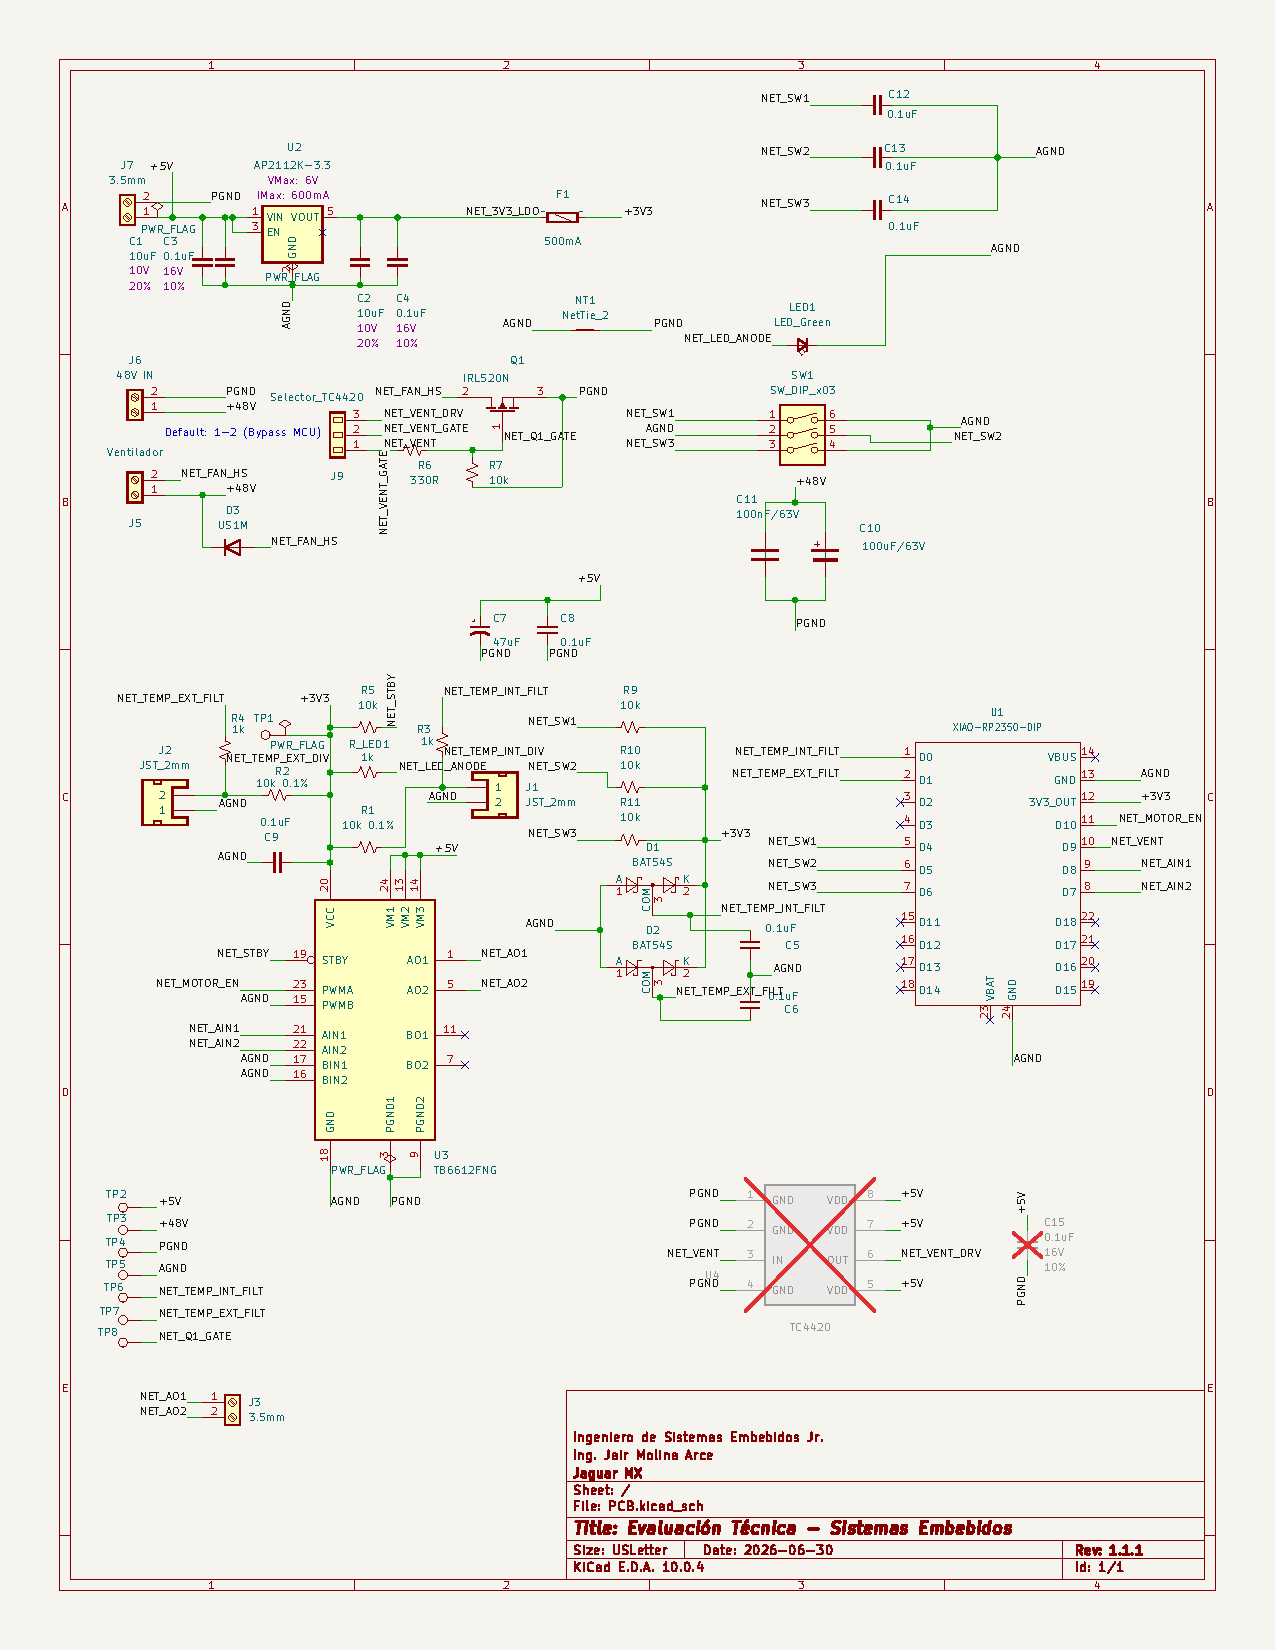
\includegraphics[width=0.95\textwidth,page=1]{img/esquematico.pdf}}
  \caption{Esquemático del sistema (KiCad). Exportado directamente del proyecto.}
\end{figure}

% =====================================================================
\section{Diseño del PCB}

\subsection{Criterios de layout aplicados}
La prioridad no fue una placa ``bonita'', sino una placa que se deje rutear sin pelear
con ella:
\begin{itemize}
  \item Bloque lógico/analógico a la izquierda ($X<149$\,mm): MCU, LDO y NTC juntos para pistas ADC cortas y limpias.
  \item Bloque de potencia a la derecha ($X>151$\,mm): U3, U4, Q1, J6, J3 y J5.
  \item \textbf{NT1 en $X=150$\,mm exacto} como frontera física y eléctrica: AGND y PGND se unen solo en ese punto controlado, siguiendo la práctica recomendada por Analog Devices para señales mixtas.
  \item Conectores y test points al borde de la placa, liberando el centro como corredor de ruteo.
  \item Desacoplos a menos de 5\,mm de su circuito integrado (C9 a $<$2\,mm de U1; C7/C8 pegados a U3; C15 junto a U4).
  \item Lazo de conmutación corto: D3 (flyback) pegado a J5 y C10/C11 (bulk) junto a la entrada J6 de 48\,V.
  \item Pistas de potencia dimensionadas a $\geq$1.5\,mm para las corrientes de \emph{stall} del actuador y del ventilador.
\end{itemize}

\subsection{Placement v4 orientado a ruteo manual}
Sobre la placa de $80\times55$\,mm (área útil $X$: 110.5--190.5\,mm; $Y$: 70.4--125.4\,mm)
se generó un placement optimizado de los 53 footprints mediante el script
\texttt{optimize\_v4.py}, con verificación automática de: presencia de los 53 refs,
cumplimiento de lados lógico/potencia, NT1 en $X=150$, límites de placa y ausencia de
solapes de courtyard con margen de 0.5\,mm. El flujo de potencia de 5\,V se lee en línea
recta (J7 $\rightarrow$ C1/C3 $\rightarrow$ U2 $\rightarrow$ C4/C2 $\rightarrow$ F1),
las cadenas NTC forman dos filas horizontales hacia el MCU y la cadena de potencia
U4 $\rightarrow$ J9 $\rightarrow$ Q1 concentra la red de gate del MOSFET.

\begin{figure}[H]
  \centering
  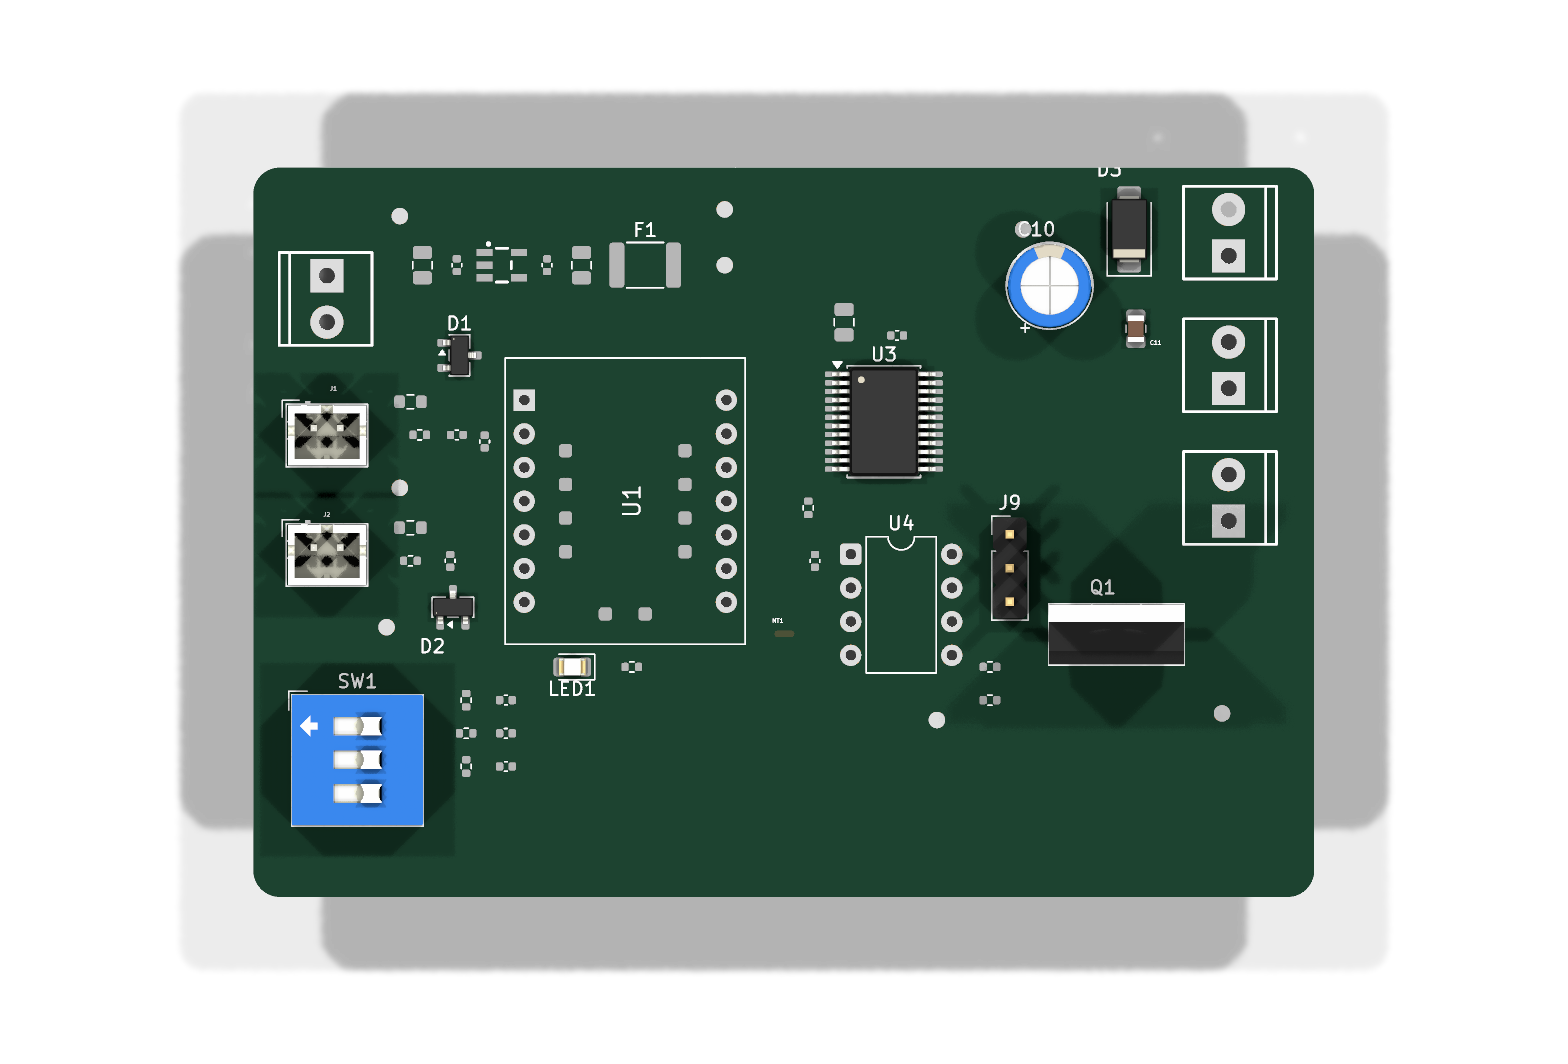
\includegraphics[width=0.92\textwidth]{img/pcb_render_top.png}
  \caption{Vista superior del PCB v4 (render KiCad): bloque lógico/analógico a la izquierda, potencia a la derecha, NT1 al centro.}
\end{figure}

\begin{figure}[H]
  \centering
  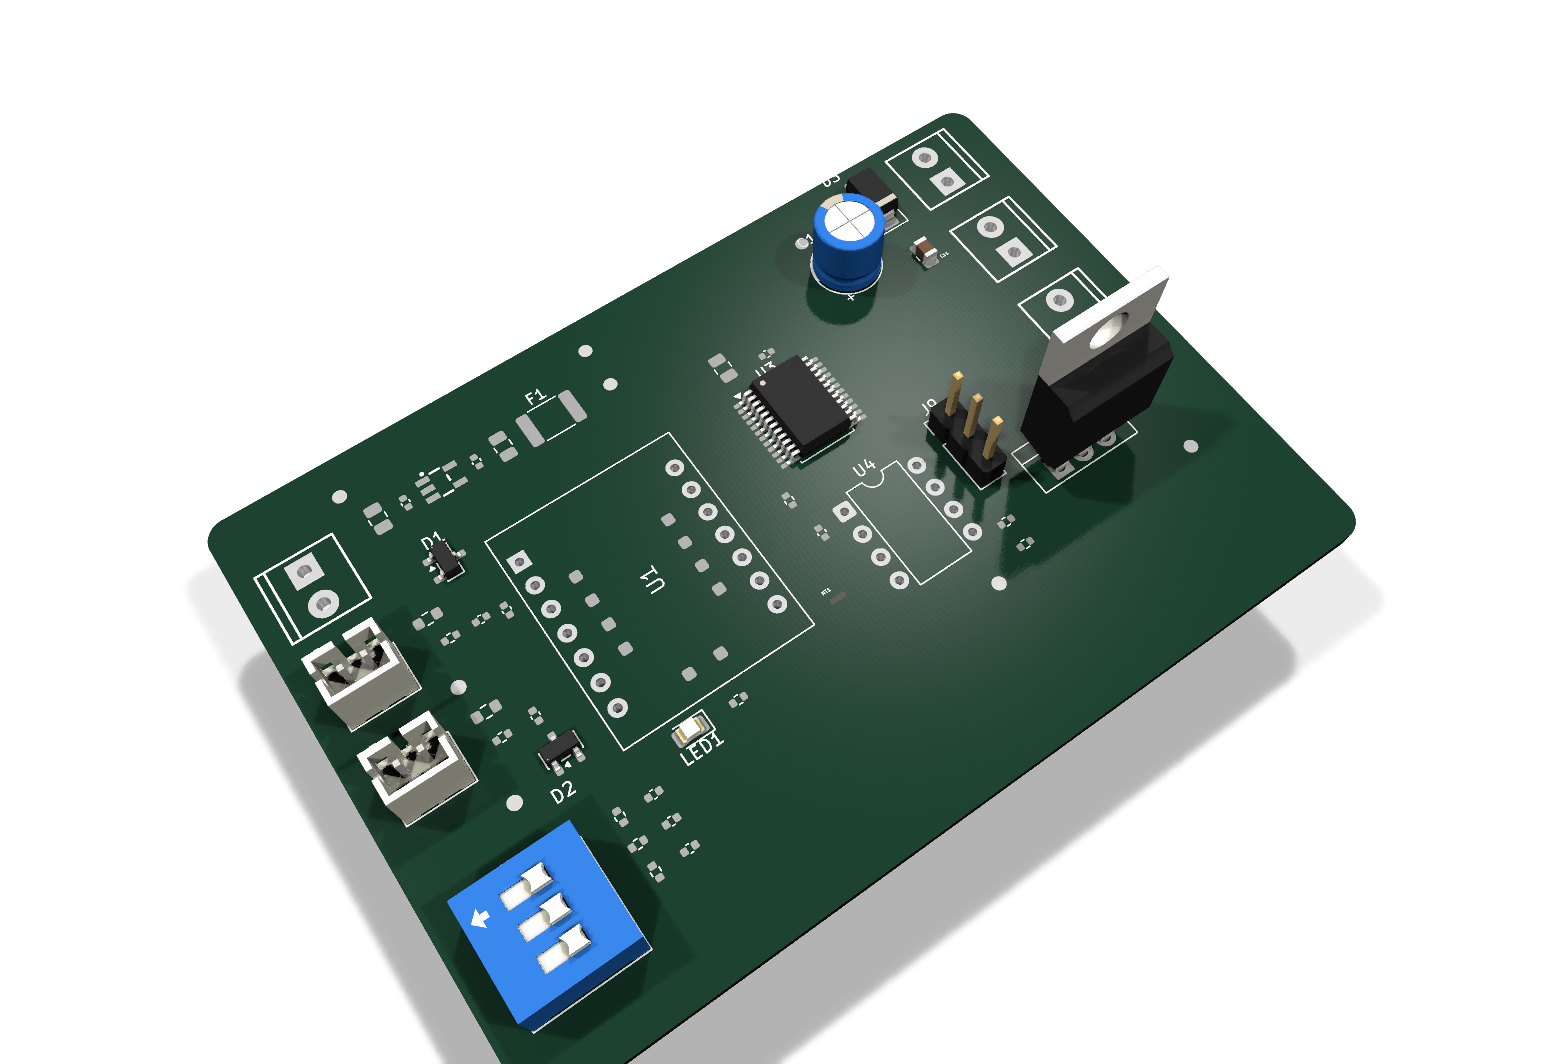
\includegraphics[width=0.92\textwidth]{img/pcb_render_iso.png}
  \caption{Vista isométrica del PCB v4. Se aprecian el DIP switch y conectores JST al borde izquierdo, el electrolítico de 48\,V, el TB6612FNG (SSOP-24) y el MOSFET TO-220 en el dominio de potencia.}
\end{figure}

% =====================================================================
\section{Decisiones Técnicas Clave}

\begin{description}[style=nextline]
  \item[Lenguaje: MicroPython] Permite iteración rápida en 4 días, acceso directo a periféricos del RP2350 (\texttt{machine.ADC}, \texttt{machine.Pin}, \texttt{machine.WDT}) y legibilidad para la sesión en vivo. El lazo de 1\,Hz no exige el rendimiento de C.
  \item[Conversión NTC: ecuación Beta] Con $B=3435$\,K la precisión es de $\pm$0.5\,°C en 0--85\,°C. Steinhart--Hart completa exigiría calibración de 3 puntos no disponible en la evaluación; la IA demostró matemáticamente que la diferencia entre ambos modelos es $<$0.5\,°C en el rango de interés.
  \item[MOSFET NMOS para 48\,V] Nivel lógico (accionable con 3.3\,V), corriente y encapsulado TO-220 soldable, con gate protegido por resistencia serie y pull-down para estado seguro sin señal.
  \item[Histéresis de $\pm$1\,°C] Evita \emph{chattering} del actuador al cruzar el setpoint, alargando la vida del mecanismo.
  \item[Control síncrono del actuador (la decisión más difícil)] El FIT0803 es de lazo abierto, sin fines de carrera. Una FSM asíncrona (\texttt{OPENING\_DAMPERS} / \texttt{CLOSING\_DAMPERS}) mantendría el lazo a 1\,Hz pero permitiría que el ventilador arrancara \emph{antes} de que las compuertas abrieran por completo, causando sobrepresión en el gabinete. Se optó por una \textbf{operación síncrona y atómica de 3\,s} con alimentación del watchdog en segundo plano: en aplicaciones industriales la predictibilidad y el \emph{fail-safe} valen más que la velocidad de respuesta.
  \item[Tierras AGND/PGND con unión única] Plano de tierra dividido por dominios y unido en un solo punto (NT1) para impedir que el ruido de conmutación de 48\,V contamine las lecturas del ADC de 12 bits.
\end{description}

% =====================================================================
\section{Uso de Inteligencia Artificial (AI Log)}
Se utilizó \textbf{Claude 3.5 Sonnet} (vía Antigravity) como asistente de revisión
estática, generación de \emph{boilerplate} y consulta de buenas prácticas. Todas las
salidas fueron auditadas; se documentan las interacciones clave:

\begin{table}[H]
\centering\footnotesize
\rowcolors{2}{RowGray}{white}
\begin{tabularx}{\textwidth}{L{2.6cm} X X}
\toprule
\rowcolor{JagDark}\color{white}\textbf{Propósito} & \color{white}\textbf{Resultado de la IA} & \color{white}\textbf{Acción del candidato} \\
\midrule
Validación del firmware (\texttt{fsm.py}, \texttt{adc\_ntc.py}) & Señaló correctamente el riesgo de expiración del WDT con el actuador activo; propuso un promedio ADC síncrono & Acepté el diagnóstico del WDT pero \textbf{rechacé} el ADC síncrono; implementé la alimentación por ráfagas en \texttt{hbridge.py} y un filtro circular asíncrono propio \\
Diseño de la simulación Wokwi & Generó el boilerplate JSON de conexiones de \texttt{diagram.json} & Revisé los GPIOs contra el requerimiento y la polaridad de los LEDs antiparalelo de \texttt{AIN1}/\texttt{AIN2} \\
Steinhart--Hart vs.\ Beta & Demostró que el error entre modelos es $<$0.5\,°C en 0--80\,°C & Elegí la ecuación Beta por menor costo computacional en el RP2040 \\
Guías de layout PCB & Sugirió planos AGND/DGND separados, unión en estrella y no cruzar potencia bajo el MCU & Apliqué los principios: pistas de 48\,V ensanchadas y entradas ADC protegidas \\
Testing con mocks & Creó \texttt{mock\_machine.py} con \texttt{Pin}, \texttt{ADC} y \texttt{WDT} & Reestructuré las pruebas para inyectar lecturas simuladas y verificar el estado \texttt{LOCKOUT} \\
\bottomrule
\end{tabularx}
\caption{Registro resumido de interacciones con la IA (30/06/2026).}
\end{table}

\subsection{Caso documentado de salida incorrecta de la IA}
La IA propuso un filtrado ADC (\texttt{\_raw\_average}) que tomaba 8 lecturas
consecutivas bloqueando el hilo dentro de \texttt{read()} ---un promedio por bloques,
no el búfer circular exigido--- y fijó los límites de error en los límites físicos del
datasheet ($-40$\,°C a 105\,°C) en lugar de los del sistema. \textbf{Detección:} al
confrontar el código con los requerimientos noté que el sistema jamás entraría en
\texttt{ERROR} si un NTC en falso contacto registraba 0\,°C. \textbf{Corrección:}
implementé manualmente un FIFO circular con una sola muestra nueva por ciclo y umbrales
de validación de 10.0\,°C a 130.0\,°C, de modo que un sensor desconectado dispare el
estado seguro de inmediato.

% =====================================================================
\section{Análisis de Confiabilidad}
Autoevaluación para entorno industrial real: \textbf{8.5/10}.

\subsection{Fortalezas}
\begin{itemize}
  \item \textbf{Arquitectura orientada a seguridad:} estados \texttt{ERROR} y \texttt{LOCKOUT}; ante falla de sensor el sistema apaga ventilador y puente H instantáneamente.
  \item \textbf{Watchdog de hardware:} reinicio automático tras 8\,s ante cuelgues o bucles infinitos, independiente del software.
  \item \textbf{Filtrado avanzado:} \emph{trimmed-mean} sobre búfer circular que descarta extremos antes de promediar, mitigando falsas alarmas por ruido.
  \item \textbf{Protecciones en hardware:} diodos flyback en cargas inductivas, clamps BAT54S en entradas ADC, fusible y desacoplo robusto.
\end{itemize}

\subsection{Debilidades identificadas (camino al 10/10)}
\begin{itemize}
  \item \textbf{Sin sensor de bloqueo mecánico:} el puente H opera por tiempo fijo a lazo abierto; una compuerta trabada implica corriente de \emph{stall} durante el tiempo restante (el TB6612FNG tiene protección térmica, pero es un punto débil mecánico).
  \item \textbf{Tolerancia a fallos de alimentación:} no hay detección proactiva de bajo voltaje ni capacitores de \emph{hold-up} que garanticen el cierre de compuertas ante pérdida de energía.
\end{itemize}

% =====================================================================
\section{Mejoras Futuras}
\begin{enumerate}
  \item \textbf{Lazo cerrado en el actuador:} fines de carrera o sensado de corriente por shunt en el puente H para detener el motor exactamente al completar el recorrido y detectar atascos.
  \item \textbf{Aislamiento galvánico:} optoacopladores entre el MCU y el gate del MOSFET de 48\,V, protegiendo al RP2350 de picos inductivos ante falla del diodo de protección.
  \item \textbf{Sensor digital redundante:} un TMP117 (I2C) en paralelo con los NTC aumentaría la confiabilidad frente al EMI de los motores, sin divisores ni calibración.
  \item \textbf{PWM con soft-start en el ventilador:} arranque gradual para reducir corrientes de \emph{inrush} y velocidad proporcional a $\Delta T = T_{int}-T_{ext}$, optimizando ruido acústico y desgaste.
\end{enumerate}

% =====================================================================
\section{Checklist de Entregables y Preparación de Fase 2}

\begin{table}[H]
\centering\small
\rowcolors{2}{RowGray}{white}
\begin{tabular}{l l l l}
\toprule
\rowcolor{JagDark}\color{white}\textbf{Entregable} & \color{white}\textbf{Contenido} & \color{white}\textbf{Ubicación en ZIP} & \color{white}\textbf{Estado} \\
\midrule
Firmware & MicroPython + README & \texttt{/firmware/} & Completo \\
Esquemático KiCad & Diseño eléctrico completo & \texttt{/kicad/*.kicad\_sch} & Completo \\
PCB KiCad & Layout + ruteo & \texttt{/kicad/*.kicad\_pcb} & Completo \\
Simulación Wokwi & URL del proyecto extendido & Sección Wokwi del .md & Completo \\
Reporte .md & Wokwi + cuestionario + AI log & \texttt{ETISEJr\_JairMolina.md} & Completo \\
ZIP final & Estructura completa & \texttt{ETISEJr\_JairMolina.zip} & Completo \\
\bottomrule
\end{tabular}
\caption{Checklist de entregables de la Fase 1.}
\end{table}

Para la sesión en vivo (2\,h) el candidato se presenta con: firmware probado y entorno
listo (Thonny / VS Code), proyecto KiCad sin errores de librería, Wokwi accesible
públicamente, cuestionario respondido y el log de IA disponible para revisión, además
del dominio de cada decisión técnica: acondicionamiento analógico, etapa de potencia,
estructura de la FSM y criterios de layout.

% =====================================================================
\section{Conclusiones}
El proyecto quedó alineado con lo solicitado por Jaguar de México. La solución integra
sensado térmico dual, decisión de control por comparación interna/externa, accionamiento
de compuertas por puente H, conmutación del ventilador de 48\,V, separación
lógica/potencia con unión única de tierras, protección y desacoplo por bloques, y una
validación apoyada en simulación, verificación automática y documentación.

Más allá del entregable, el desarrollo reprodujo un flujo real de ingeniería: entender
el requerimiento, traducirlo a arquitectura y esquema, acomodar la placa pensando en
quien la va a rutear y depurar, validar contra los casos de borde, corregir con criterio
---incluso frente a las sugerencias de la IA--- y dejar todo listo para entrega. Las
lecciones principales: un NTC analógico merece el mismo rigor en layout que en cálculo;
el TB6612FNG rinde solo si su desacoplo y ubicación se toman en serio; la etapa de 48\,V
exige su propio dominio y criterio de protección; y la documentación debe contar la
misma historia que el esquemático, el PCB y el firmware.

\vspace{1.2cm}
\begin{flushright}
\begin{tabular}{c}
\rule{6cm}{0.4pt}\\
\textbf{Ing. Jair Molina Arce}\\
Candidato --- Ingeniero de Sistemas Embebidos Jr.\\
Jaguar de México --- Julio de 2026
\end{tabular}
\end{flushright}

\end{document}
